\documentclass[11pt] {article}
\usepackage{amssymb}
\usepackage{amsmath}
\usepackage[colorlinks=true]{hyperref}
\usepackage[scaled=2.5]{helvet}
\setlength{\parsep}{20pt}
\usepackage{geometry}
\geometry{letterpaper}
\usepackage{graphicx}
\usepackage{amssymb}
\usepackage{caption}
\usepackage{subcaption}
\usepackage{enumerate}

\newcommand{\bs}[1] {\boldsymbol{#1}}

\begin{document}
\title{Regularized variational fracture modeling}
\author{V.Kaushik}
%\date{January 12, 2015}
\maketitle
\section{Introduction}
Computational modeling of crack initiation and propagation continues to be an active area of research. Griffith developed the necessary condition for crack initiation using energy based arguments by considering the contribution of both bulk energy (elastic strain energy) and surface energy (see \cite{griffith_1921}). Griffith postulated that for a crack to initiate the total energy needs to be minimized with respect to a virtual crack extension. George Irwin reformulated the Griffith theory to introduce the concept of energy release rate ($G$) and showed that crack would initiate if $G \ge G_c$, where $G_c$ is the fracture toughness of the material (see \cite{irwin_1997}). However, Griffiths condition is not a sufficient one for crack growth and thus, leading to proposition of numerous crack propagation criteria. Some of the classical crack propagation criteria for the crack to kink at an angle $\theta_c$ at the crack tip with respect to the straight crack propagation direction are:
\begin{itemize}
	\item Criterion of maximum circumferential stress was proposed by Erdogan and Sih (see \cite{erdogan_1963}) where the crack is assumed to initiate when $\sigma_{\theta \theta}$ reaches a critical value $\sigma_c$ (which can be calibrated based on $G_c$). The kink angle $\theta_c$ can be derived based on $\frac{\partial \sigma_{\theta \theta}}{\partial \theta}\big|_{\theta=\theta_c} = 0$ and $\frac{\partial^2 \sigma_{\theta \theta}}{\partial^2 \theta}\big|_{\theta=\theta_c} < 0$ such that it is perpendicular to $\sigma_{\theta \theta}\big|_{\theta = \theta_c}$ direction.
	\item Criterion of maximum energy release rate (MERR) was proposed by Hussain et al. (see \cite{hussain_1974}) where crack initiation follows the Griffith criterion ($G \ge G_c$) and the propagation direction is decided when $\frac{\partial G}{\partial \theta}\big|_{\theta=\theta_c} = 0$ and $\frac{\partial^2 G}{\partial^2 \theta}\big|_{\theta=\theta_c} < 0$.
	\item Criterion of strain energy density was proposed by Sih (see \cite{sih_1974}) where the singular strain energy density ($U(\theta)$) depends on the angular distribution $\theta$. The crack initiates when $U=U_c$, where $U_c$ is the critical strain energy density (which can be calibrated based on $G_c$) and propagates when $\frac{\partial U(\theta)}{\partial \theta}\big|_{\theta=\theta_c} = 0$ and $\frac{\partial^2 U(\theta)}{\partial^2 \theta}\big|_{\theta=\theta_c}  < 0$.
	\item The principle of local symmetry is a crack propagation criterion proposed by Banichuk (see \cite{banichuk_1970}), Goldstein and Salganik (see \cite{goldshtein_1970,gol_1974}), where the crack initiates based on the Griffith criterion and propagates in the direction of mode-II stress intensity factor $K_{II}=0$.
	\item Criterion of maximum principal stress is a crack propagation criterion proposed by Maiti and Smith (see \cite{maiti_1984}), where crack initiates based on the Griffith criteria and propagates perpendicular to the direction of maximum principal stress.
\end{itemize}
Crack propagation criteria were developed primarily to predict crack paths which are curvilinear due to asymmetric stress fields. Amongst the criteria listed above it has been observed in experiments, specifically mode-II failure that the crack kinks based on $K_{II} = 0$ criterion (see \cite{buzzard_1986,smith_1972}). Cotterell and Rice (see \cite{cotterell_1980}) proposed a first order (with respect to the kink angle) solution for stress intensity factors (SIFs) for infinitesimally small and finite length kinked cracks. For small kink angles they have also derived an equation for the crack path such that the crack would follow the criterion $K_{II} = 0$. However, some studies by Asher Rubinstein have shown that crack path does not follow any of the above mentioned criteria (see \cite{rubinstein_1991}). The author analyzed the SIFs at different stages of crack growth using experimental data of crack paths in a polystyrene single notch specimen with a hole positioned at an angle to the notch tip. It was seen that along the crack path $K_{II}$ varied up to a maximum of $5\%$ of $K_I$ (mode-I stress intensity factor) and the author proposed that turning of the crack is governed by $\frac{\partial G}{\partial \theta}\big|_{\theta = \theta_c} = G_{\theta c}$, where $G_{\theta c}$ is a material constant. This indicates that there is no clear consensus on the choice of crack propagation criteria in brittle materials.

\section{Regularized variational fracture modeling}
One of recent developments in computational fracture mechanics has been the emergence of variational fracture method to predict crack paths in elastic materials. This method was introduced by Francfort and Marigo (see \cite{francfort_1998}) as a generalization of Griffith theory of brittle fracture. In this method, crack growth is evolved such that the total energy (sum of bulk and surface energies) of the system is minimized. Francfort and co-workers have advocated this method as a global minimization problem such that the crack and global displacement field will evolve to globally minimize the total energy. We, however, do not adopt this point of view and consider crack growth in a sequence of infinitesimal increments where the direction of crack growth reduces the total energy as much as possible. Thus, the system always moves in the direction of local energy gradient. The energy functional introduced by Francfort and Marigo over a domain $\Omega \subset \mathbb{R}^2$ and a sufficiently smooth crack set $\Gamma \subset \mathbb{R}^1$ is given by,
\begin{align}\label{FM}
\Psi (\bs u, \Gamma) = \int_{\Omega \setminus \Gamma} \psi_e\left(\bs \nabla \bs u\right) d\Omega + \int_{\Gamma} G_c d\Gamma,
\end{align}
where $\bs{u}$ is the displacement field, $\psi_e\left(\bs \nabla \bs u\right)$ is the elastic strain energy and $G_c$ is the bulk fracture toughness. It can be clearly seen from the eq.~\eqref{FM} that the energy functional $\Psi$ consists of evolving volume ($\Omega \setminus \Gamma$) and surface ($\Gamma$) integrals and numerically tracking evolution of $\Gamma$ is difficult. To circumvent this problem, the surface integral on $G_c$ in eq.~\eqref{FM} was approximated by an equivalent regularized form (see \cite{bourdin_2000,miehe_2010,borden_2012} for more details) and the regularized variational fracture model (RVFM) is given as,
\begin{align}
\int_{\Gamma} G_c d\Gamma \approx \int_{\Omega}\frac{G_c}{2} \left(\ell_0\| \bs \nabla \phi \|^2 +\frac{\phi^2}{\ell_0}\right) d\Omega \nonumber,
\end{align}
and therefore, the modified energy functional $\Psi_\epsilon(\bs u, \phi)$ is
\begin{align}\label{PFM}
\Psi_\epsilon(\bs u, \phi) = \int_{\Omega}g(\phi) \psi_e\left(\bs \nabla \bs u\right) d\Omega + \int_{\Omega}\frac{G_c}{2} \left(\ell_0\| \bs \nabla \phi \|^2 +\frac{\phi^2}{\ell_0}\right) d\Omega.
\end{align}
The symbol $\phi$ is a scalar damage variable, $g(\phi)$ is a degradation function, $\ell_0$ is the length scale parameter of the model and $\|\cdot\|$ is the Euclidean-2 norm. The damage variable $\phi$ introduces fracture into the model and it is bounded between 0 and 1. The solid is unbroken when $\phi = 0$ and is completely broken when $\phi = 1$. The regularized model approaches the variational fracture model proposed by Francfort and Marigo (see eq.~\eqref{FM}) as the length scale parameter $\ell_0 \to 0$.
\par
The RVFM given by eq.~\eqref{PFM} is very similar to the phase field model proposed by Karma et al. (see \cite{karma_2001}) and retains central idea that crack evolution occurs in the direction of local energy gradient. Therefore, the crack growth law emerges naturally from the variational formalism as given by Hakim and Karma (see \cite{hakim_2009}). Let the crack deviate from the straight crack path by $\delta \theta$ for an arbitrary loading then it satisfies the following conditions,
\begin{enumerate}[1)]
	\item Crack initiation occurs as per Griffith criterion i.e, $G=G_c$.
	\item Crack growth occurs $G_\theta = 2 \gamma_\theta$, where $G_\theta = \frac{\partial G}{\partial \theta}$, $\gamma_\theta = \frac{\partial \gamma (\theta)}{\partial \theta}$ and $\gamma(\theta)$ is the anisotropic surface energy.
\end{enumerate}
It can be noted from the second postulate that when the surface energy is isotropic $\left(\frac{\partial \gamma (\theta)}{\partial \theta} = 0\right)$, the criterion of crack growth is identical to MERR criterion.

\section{Preliminary results}
In a number of cases RVFM predicts the crack path that is observed in experiments and that predicted by using the maximum energy relase rate fracture criterion in simple linear elastic fracture mechanics problems.
\begin{enumerate}[1.]
	\item RVFM is a generalized Griffith model, therefore we can verify that crack initiation occurs at $G=G_c$ which can be seen in Fig.~\ref{Fig1} for edge notched geometry subjected to far-field stress $\sigma^\infty$. In the finite element simulations the height of the geometry is chosen to be much larger than the width $b$. For details on evaluating energy release rate $G$ for this geometry refer to \cite{kuhn_2010}.
	\item In simple RVFM problems, RVFM produces crack trajectories predicted by MERR criterion such as for a geometry subjected to mode-II shear shown in Fig.~\ref{Fig2}. It can be seen that crack initiation occurs at $21.4^o$ with respect to (w.r.t) the x-axis and which from MERR criterion is equal to $19.5^o$ (see \cite{kuna_2013}).
	\item RVFM has also shown good comparison against experimental crack paths such as for a notched plate with 3 holes which can be seen in Fig.~\ref{Fig3}.
\end{enumerate}
\begin{figure}
	\centering
	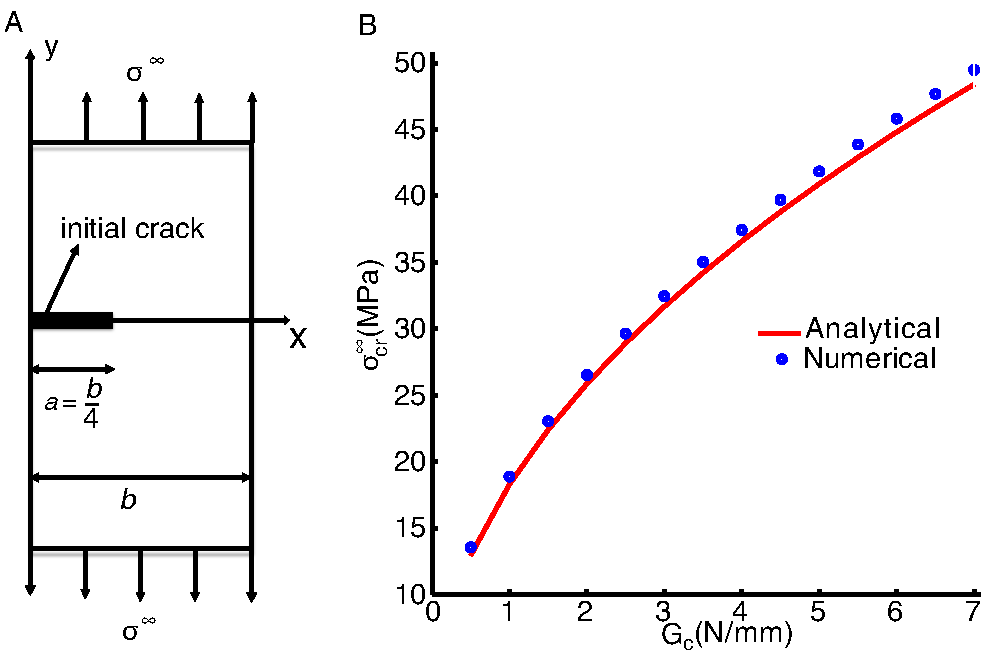
\includegraphics[width=\textwidth]{./Fig1.pdf}
	\caption{(A) This is a schematic of edge-crack geometry subjected to far-field stress $\sigma^\infty$. The initial crack length is $a$, the width of the geometry is $b$. The initial crack length $a$ = $b/4$. (B) Toughness ($G_c$) from finite element simulations for the edge-crack geometry given in Fig.~1(A) is plotted in this figure against the far field stress ($\sigma_{cr}^{\infty}$) at which crack initiates. }
	\label{Fig1}
\end{figure}
\begin{figure}
	\centering
	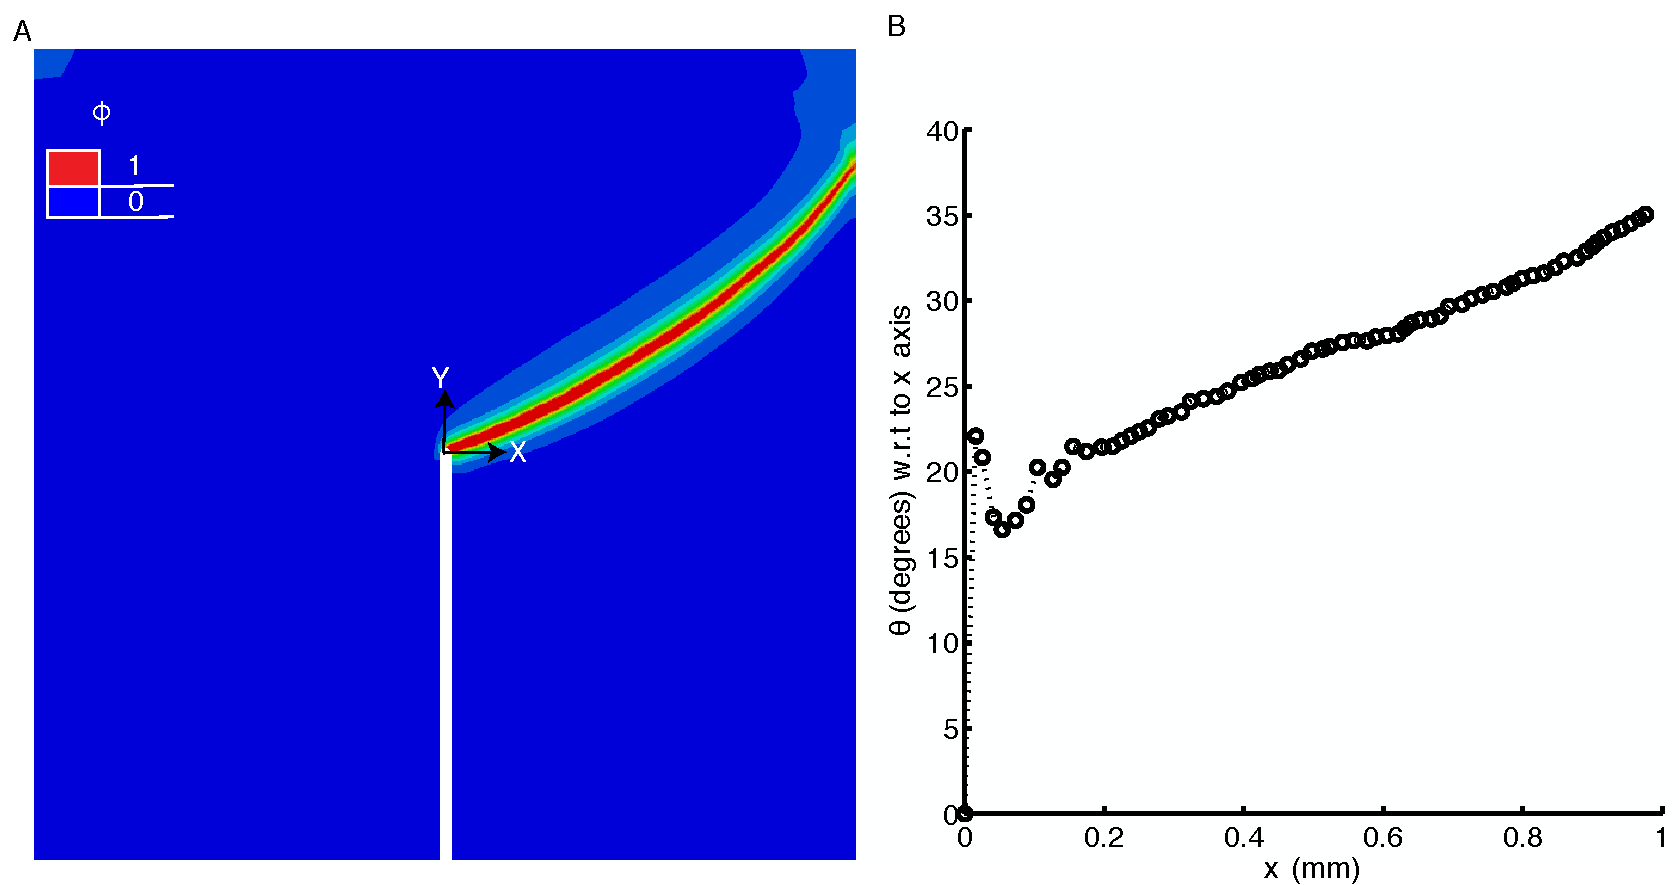
\includegraphics[width=1\textwidth]{./Fig2.pdf}
	\caption{(A) This figure shows the contour plot of the damage field $\phi$ with $\phi=1$ being the fractured region and it can be seen that crack kinks at an angle from the x-axis when the geometry is subjected to pure shear parallel to $y$ axis. (B) On extracting the crack path from the contour plot it can be seen that the crack initiation angle is $21.4^o$ which compares well against MERR value of $19.5^o$.}
	\label{Fig2}
\end{figure}
\begin{figure}
	\centering
	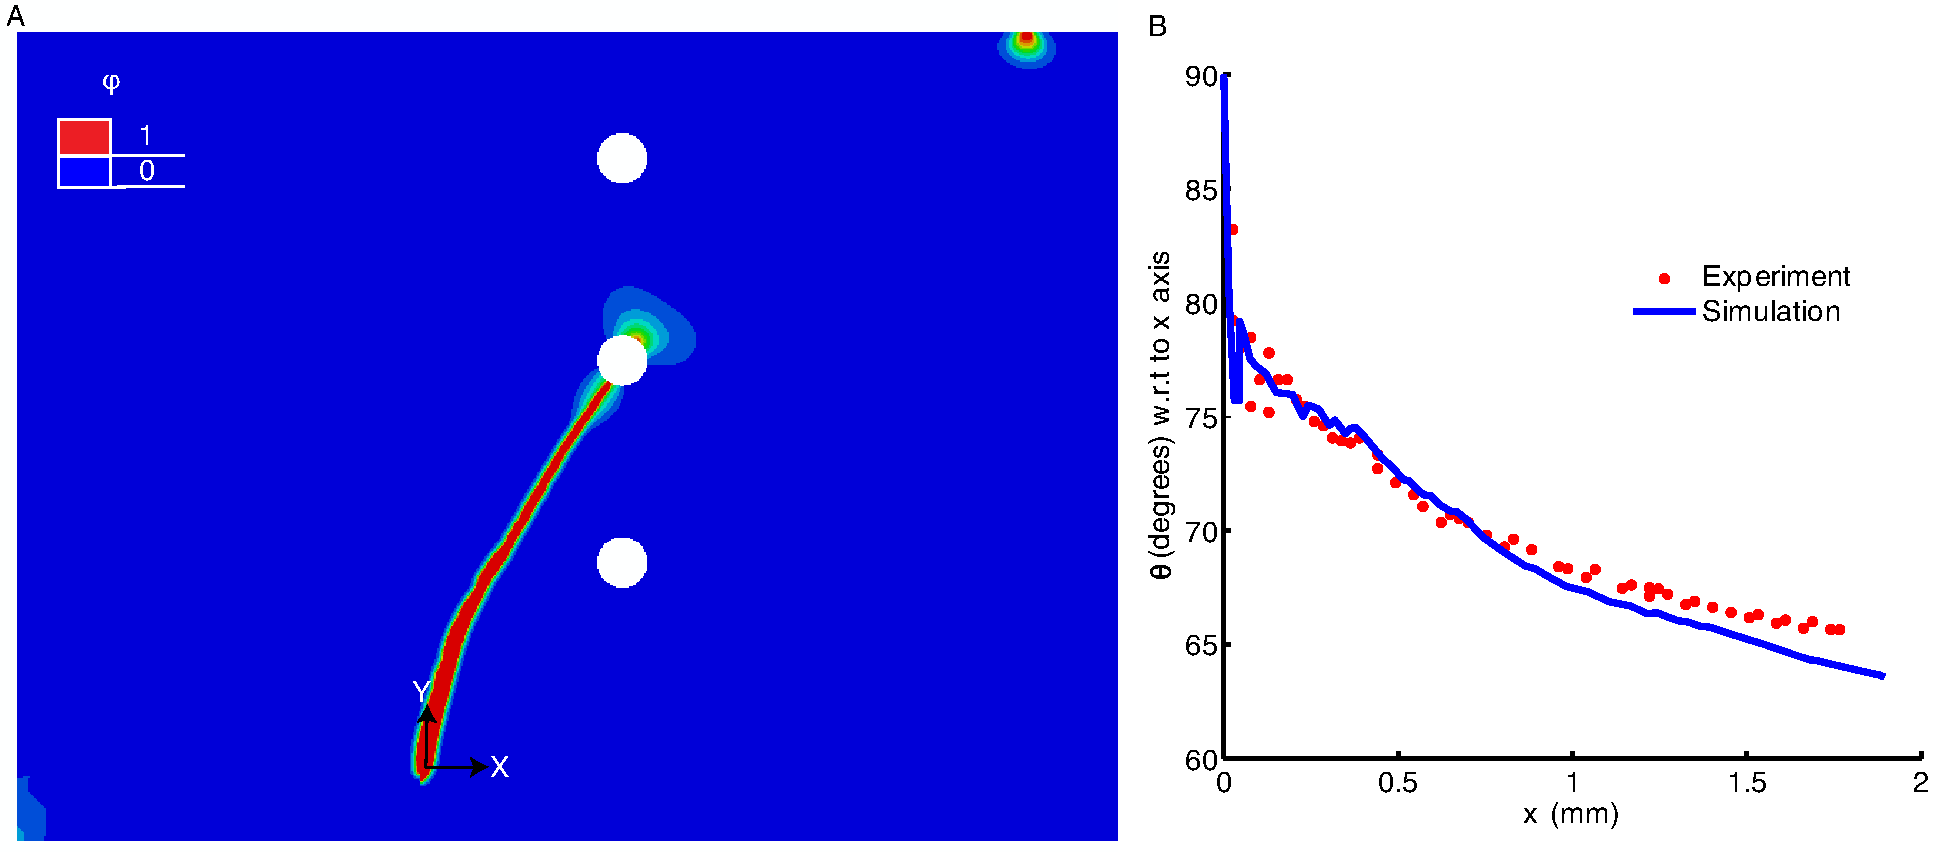
\includegraphics[width=\textwidth]{./Fig3.pdf}
	\caption{(A) This figure shows the contour plot of the damage field $\phi$ with $\phi=1$ is the fractured region. (B) On extracting the crack path from the contour plot and from the experimental data (see \cite{bittencourt_1996}) it can be seen that the crack paths compare fairly well.}
	\label{Fig3}
\end{figure}
In comparison to comparable computational methods the RVFM has the following very attractive features.
\begin{enumerate}[(i)]
	\item There is no need to remesh the solid after each crack increment.
	\item It can handle a variety of complex crack
	patterns, such as branched and intersecting cracks (see Fig.~\ref{Fig4}).
	\item There is no need for a priori knowledge about the general shape and topology of the crack pattern.
	\item No special treatment is needed for handling cracks patterns in 3D solids.
\end{enumerate}
\begin{figure}
	\centering
	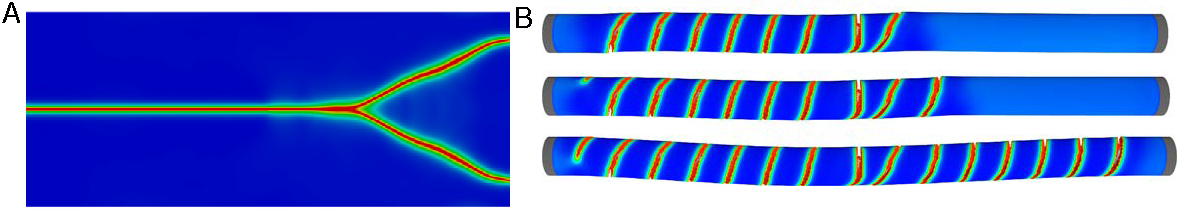
\includegraphics[width=1.0\textwidth]{./Fig4.pdf}
	\caption{(A) The phenomenon of crack branching seen in glass under dynamic loads is captured using RVFM (see \cite{borden_2012} for more details). (B) Multicracking in a brittle cylinder under uniaxial tension (see \cite{bourdin_2008} for more details). }
	\label{Fig4}
\end{figure}
The primary drawback of RVFM is the computational cost. The size of the finite elements,$h$, need to be smaller (typically $<$ 1/10 ) than $\ell_0$, the regularization parameter. The parameter $\ell_0$ dictates the region over which the crack is smeared out. For that reason $\ell_0$ needs to be much smaller ($<$ 1/10 ) than the smallest of the characteristic geometric parameters of the crack. In sharp notches the notch tip radius is at least 1/50 of the solid dimensions.
Thus, for accurate calculation typical RVFM simulation typically contain 0.1–1 million elements. However, we do not perceive this as a significant drawback. For example the simulations reported in section X were based on FE meshes that contained 500,000 elements. This was possible because the computational simulations being developed
by the PI’s group are capable of running on several CPUs in parallel. The PI has access to significant computational resources at Brown. See section XX for details.
\par
A number of computational techniques have been developed and are routinely used to model fracture. These can broadly be classified into:
\begin{enumerate}[(i)]
	\item Finite element (FE) based,
	\item Boundary element (BE) based,
	\item Singular integral equation based,
	\item Molecular Dynamics and Statics based methods.
\end{enumerate}
Finite element based computational methods provide some useful advantages over some of the other methods. Over the past years
several computational techniques have been developed to model crack growth in materials. The most popular of these are:
\begin{enumerate}
	\item Cohesive zone method (CZM) \cite{xu_1994,camacho_1996},
	\item Extended finite element method (XFEM) \cite{dolbow_1999},
	\item Use of Singularity elements,
	\item Element deletion methods,
	\item Virtual Internal Bond method.
\end{enumerate}
CZM is based on finite element analysis. Crack growth is modeled by allowing the adjoining elements ahead of the crack tip to separate. As the elements separate, tractions act on the mating faces of the element as per a pre assigned traction separation law (cohesive zone law). When the separation reaches a critical value, the mutual traction vanishes and the element are taken to have completely separated and are now part of the opposing crack faces. As the RVFM, in CZM there is no need for remeshing the domain after each growth increment. Furthermore, its is also possible to handle branched and intersecting cracks. However, the CZM has the following drawbacks in
comparison to RVFM:
\begin{enumerate}[a.]
	\item \textit{Mesh sensitivity}: crack trajectory depends critically on the size of finite elements, especially in regions close to the crack propagation.
	\item Need of \textit{a priori} knowledge of crack growth direction: The crack can only grow in the directions in which the modeler has chosen to allow adjoining pairs of elements to separate. So, insufficient \textit{a priori} knowledge about the crack growth direction can cause the CZM to predict incorrect crack paths. Allowing all pairs of adjoining elements to separate is not a viable solution, since that substantially changes the bulk mechanical behavior of the solid.
\end{enumerate}
XFEM is also based on finite element method. In XFEM the standard finite element basis functions are enriched (“extended”) by including basis functions that allow displacement fields to be discontinuous across elements. As in RVFM, in XFEM too there is no need for remeshing. Also as in RVFM, there is no critical need of \textit{a priori knowledge} of the crack growth. As in RVFM, it is also capable of handle branched and intersecting cracks through some
modifications. However these modifications are not straightforward since they include adding different types of basis function depending on the topology of crack patterns, e.g. on the
number of branches. Further, to model the displacement discontinuity introduced during crack propagation discontinuous enriched elements are used. Introduction of these enriched elements can considerably increase the condition number of the linear system of equations being solved, thus, making the system of linear equations illconditioned
which leads to serious convergence problems (see \cite{lasry_2010}). Hence, it is often necessary to come up with strategies to prevent illconditioning while using XFEM (see \cite{xiao_2007l,zhao_2014}). Modeling complex crack patterns such as crack branching with high accuracy is not feasible with these methods (see \cite{song_2008}).
\par
The advantages of the RVFM:
\begin{enumerate}[(i)]
	\item It has been demonstrated that this model has the capability to model the formation and evolution of complex crack patterns such as crack branching in a straightforward manner (see \cite{borden_2012} for more details).
	\item It has also been shown that crack paths produced in experiments can be accurately reproduced (see Fig.~\ref{Fig3}).
	\item The length scale parameter $\ell_0$ eliminates the dependence of crack path on element size (see \cite{miehe_2010,borden_2012}).
\end{enumerate}

\bibliographystyle{plain}
\bibliography{PFM}
\end{document}
